\documentclass[aspectratio=169]{beamer}

\usepackage{amsmath,amssymb}
\usepackage{booktabs}
\usepackage{tabularx}
\usepackage{tikz}
\usetikzlibrary{arrows.meta,backgrounds,calc,positioning,shapes.multipart}
\usepackage[english, polish, main=brazilian]{babel}
\usepackage{ragged2e}
\usepackage{csquotes}
\usepackage[
  backend=biber,
  style=authoryear,
  maxcitenames=2,
  doi=false,
  isbn=false,
  url=true
]{biblatex}
\addbibresource{refs.bib}

\definecolor{cookieDemoBlue}{HTML}{356AE6}
\usetheme[
  accent=cookieDemoBlue,
  progressbar=foot,
  sectionpage=progressbar,
  subsectionpage=progressbar,
  numbering=fraction,
  numberrail=subsection,
  block=fill,
  notes=show, % Aqui
  toc=aftertitle,
  closing=contact
]{cookie}

\lstset{style=cookie}

\title[Cores]{Cores em Computação Gráfica}
\subtitle{Integrando a Percepção Humana, Modelos Matemáticos e Implementação em OpenGL}
\author[Júlio \& Luiz]{Júlio C. Oliveira \\ Luiz G. Moreira}
% \cookieemail{seniormars@rice.edu}
\institute{Icen}
\cookieuni{Universidade Federal do Pará}
\cookielocation{Belém, Pará}
\date{\today}
% \cookietagline{A small theme for modern slides}
\cookietitleimage{assets/cookie-background.png}
\cookieclosingtitle{Obrigado}
\cookieclosingtext{Perguntas?}
% \cookieclosingqr{https://example.org/cookie-beamer}
% \cookieclosingqrlabel{Replace with your project URL}

\titlegraphic{%
  \begin{tikzpicture}[scale=.70]
    \fill[white,opacity=.94] (0,0) circle[radius=1.15];
    \fill[cookieDemoBlue!82!black] (-.43,.40) circle[radius=.12];
    \fill[cookieDemoBlue!82!black] (.36,.50) circle[radius=.10];
    \fill[cookieDemoBlue!82!black] (.52,-.22) circle[radius=.13];
    \fill[cookieDemoBlue!82!black] (-.38,-.43) circle[radius=.09];
    \fill[cookieDemoBlue!82!black] (.02,.02) circle[radius=.11];
  \end{tikzpicture}%
}

\newsavebox{\cookieDemoPenguin}
\savebox{\cookieDemoPenguin}{\cookiepenguin[scale=.31]}
\newcommand{\cookiedemomathcomparisonbody}{%
  \footnotesize
  \setlength{\abovedisplayskip}{.24em}%
  \setlength{\belowdisplayskip}{.24em}%
  \begin{columns}[T,onlytextwidth]
    \column{.18\textwidth}
      \centering
      \cookiekicker{Lining}\par
      \vspace{.45em}
      1234567890

    \column{.18\textwidth}
      \centering
      \cookiekicker{Oldstyle}\par
      \vspace{.45em}
      \oldstylenums{1234567890}

    \column{.22\textwidth}
      \centering
      \cookiekicker{Accents}\par
      \vspace{.45em}
      $\hat{x},\;\check{x},\;\tilde{a},\;\bar{a},\;\dot{y},\;\ddot{y}$

    \column{.36\textwidth}
      \centering
      \cookiekicker{Differentials}\par
      \vspace{.45em}
      $\displaystyle \iiint f(x,y,z)\,\mathrm dx\,\mathrm dy\,\mathrm dz$
  \end{columns}

  \vspace{.30em}
  \begin{columns}[c,onlytextwidth]
    \column{.47\textwidth}
      \[
        \frac{1}{\displaystyle 1+
          \frac{1}{\displaystyle 2+
          \frac{1}{\displaystyle 3+x}}}
        +
        \frac{1}{1+\frac{1}{2+\frac{1}{3+x}}}
      \]

    \column{.47\textwidth}
      \[
        F:\left|\begin{array}{ccc}
          F''_{xx} & F''_{xy} & F'_x \\
          F''_{yx} & F''_{yy} & F'_y \\
          F'_x     & F'_y     & 0
        \end{array}\right|=0
      \]
  \end{columns}

  \vspace{.02em}
  \begin{columns}[c,onlytextwidth]
    \column{.30\textwidth}
      \[
        \mathop{\int\!\!\!\int}_{\mathbf{x}\in\mathbb R^2}
        \!\langle \mathbf{x},\mathbf{y}\rangle\,\mathrm d\mathbf{x}
      \]

    \column{.34\textwidth}
      \[
        \overline{\overline{a\alpha}^2+\underline{b\beta}
        +\overline{\overline{d\delta}}}
      \]

    \column{.30\textwidth}
      \[
        \left]0,1\right[+\lceil x\rfloor-\langle x,y\rangle
      \]
  \end{columns}

  \vspace{.05em}
  \begin{columns}[c,onlytextwidth]
    \column{.44\textwidth}
      \[
        \begin{aligned}
          e^x &\approx 1+x+x^2/2! \\
              &\quad{}+x^3/3!+x^4/4!
        \end{aligned}
      \]

    \column{.50\textwidth}
      \[
        \binom{n+1}{k}=\binom{n}{k}+\binom{n}{k-1}
      \]
  \end{columns}

  \vspace{-.15em}
  {\scriptsize
  \[
    \begin{aligned}
      p(R,\phi)
      &\sim \int_{-\infty}^{\infty}
      \frac{
        \tilde{W}_n(\gamma)
        \exp\!\left[
          \imath R/a
          \left(\sqrt{k^2a^2-\gamma^2}\cos\phi\right)
        \right]
      }{
        \left(k^2a^2-\gamma^2\right)^{3/4}
      }\\[-.15em]
      &\qquad{}\times
      \frac{1}{
        {H_n^{\prime}}_n^{(1)}
        \left(\sqrt{k^2a^2-\gamma^2}\right)
      }\,d\gamma .
    \end{aligned}
  \]
  }%
}
\begin{document}

\maketitle

% ==========================================
% SEÇÃO 1: INTRODUÇÃO E FÍSICA DA LUZ
% ==========================================
\section{Introdução}

\begin{frame}{Percepção Humana}
    \begin{columns}
        \begin{column}{0.45\textwidth}
            \begin{itemize}
                \item \textbf{Fotorreceptores na Retina:}
                \begin{itemize}
                    \item Bastonetes ($\approx$ 125 milhões).
                    \item Cones ($\approx$ 6 a 7 milhões).
                \end{itemize}
                \vspace{0.3cm}
                \item \textbf{Teoria Tricromática:}
                \begin{itemize}
                    \item Azul.
                    \item Verde.
                    \item Vermelho/Amarelo.
                \end{itemize}
            \end{itemize}
        \end{column}
        
        \begin{column}{0.55\textwidth}
            \begin{figure}
                \centering
                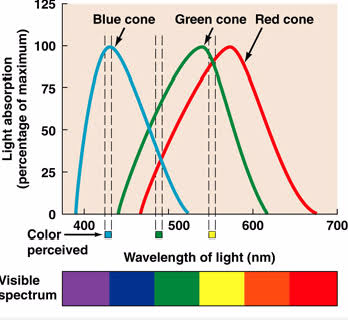
\includegraphics[width=0.75\textwidth]{images/curvas_sensibilidade_cones.jpg}
                \caption{Curvas de resposta espectral dos cones S, M e L.}
            \end{figure}
        \end{column}
    \end{columns}

    \note{
        A retina funciona com base em dois tipos de receptores:

        \begin{enumerate}
            \item \textbf{Bastonetes ($\approx$ 125 milhões):} São sensores de alta sensibilidade, mas monocromáticos. Eles não detectam cor, apenas intensidade luminosa. É a nossa visão noturna.
            
            \item \textbf{Cones ($\approx$ 6 a 7 milhões):} São os sensores responsáveis pela cor, mas que só funcionam bem com bastante luz. Note que nós temos muito menos sensores de cor do que de brilho.
        \end{enumerate}
        
        O gráfico ilustra a Teoria Tricromática, que é a base para a existência do RGB nos computadores. Nós não temos um cone para cada cor existente; a gente tem três tipos de cones (curtos: detectam azul. médios: detectam verde. longos: detectam vermelho/amarelo.), e o cérebro faz uma média ponderada dos sinais recebidos por eles.
    }
\end{frame}

\begin{frame}{Colorimetria}
    \begin{columns}
        \begin{column}{0.45\textwidth}
            \begin{figure}[H]
                \centering
                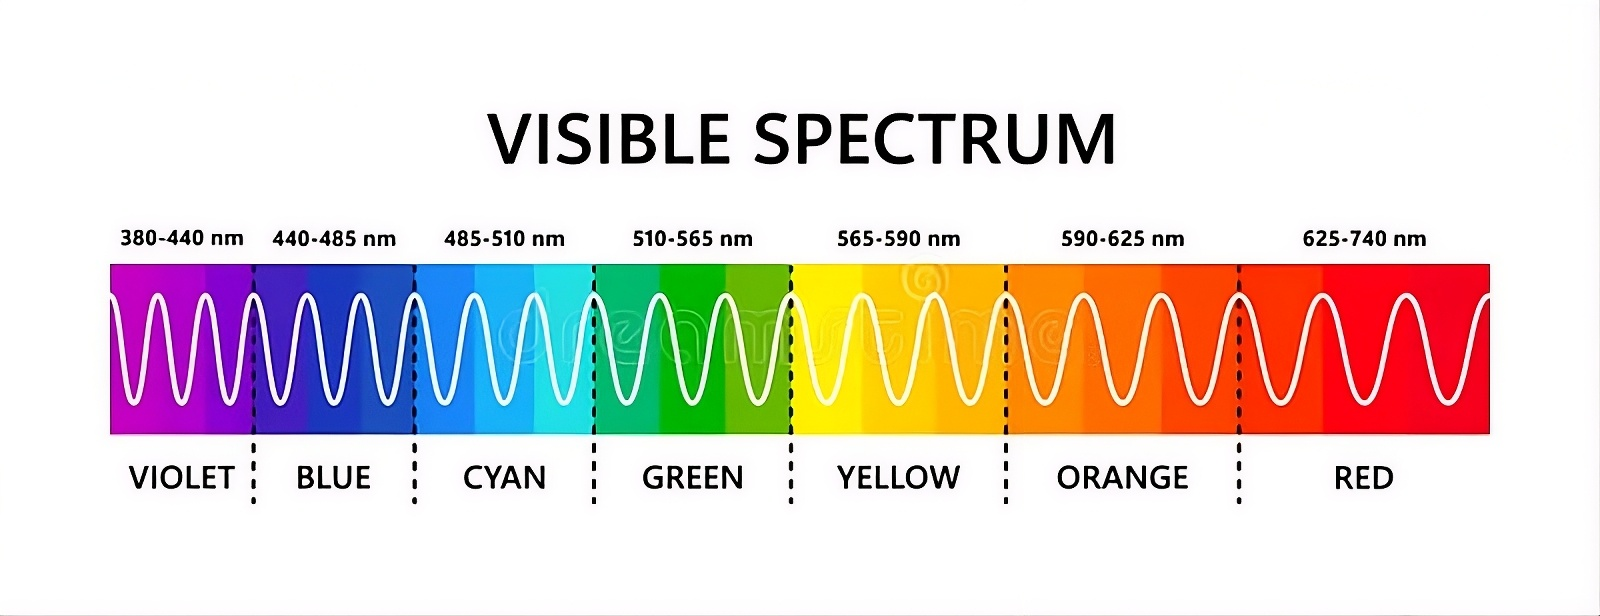
\includegraphics[width=1\textwidth]{images/visible_spectrum.jpg}
                \caption{Espectro eletromagnético.}
            \end{figure}
        \end{column}    

        \begin{column}{0.55\textwidth}
            \textbf{Parâmetros da Colorimetria:}
            \begin{itemize}
                \item Matiz (Hue).
                \item Saturação.
                \item Brilho / Intensidade.
            \end{itemize}
        \end{column}    
    \end{columns}

    \begin{exampleblock}{Aberração Cromática}
        Evitar o uso simultâneo de cores nos extremos opostos do espectro \\(ex: Vermelho Puro + Azul Puro).
    \end{exampleblock}

    \note{
        \begin{columns}[T]
            \begin{column}{0.5\textwidth}
                \scriptsize
                \textbf{Física e Colorimetria:}
                \begin{itemize}
                    \item \textbf{Espectro:} 380 nm (violeta/alta freq) a 750 nm (vermelho/baixa freq).
                    \item \textbf{Matiz (Hue):} Comprimento de onda dominante (o nome da cor).
                    \item \textbf{Saturação:} Pureza da cor (onda pura vs. misturada com luz branca).
                    \item \textbf{Brilho:} Energia luminosa total ($\int$ área sob a curva espectral).
                \end{itemize}
            \end{column}

            \begin{column}{0.5\textwidth}    
                \scriptsize
                \textbf{Aberração Cromática (UI/UX):}
                \begin{itemize}
                    \item \textbf{Refração:} Cristalino dobra cores de forma diferente.
                    \item \textbf{Azul (curta):} Dobra mais, foco à frente.
                    \item \textbf{Vermelho (longa):} Dobra menos, foco ao fundo.
                    \item \textbf{Interface (Pane):} Texto azul em fundo vermelho força o olho a contrair/relaxar o músculo freneticamente para focar no mesmo plano.
                    \item \textbf{Efeito:} Fadiga visual extrema e dor de cabeça em minutos.
                \end{itemize}
            \end{column}
        \end{columns}
    }
\end{frame}
% ==========================================
% SEÇÃO 2: SÍNTESE DE CORES: RGB VS. CMYK
% ==========================================
\section{Síntese de Cores}
\begin{frame}{Síntese Aditiva: Modelo RGB}
    \begin{columns}[T]
        \begin{column}{0.55\textwidth}
            \begin{itemize}
                \item \textbf{Sistemas Aditivos de Emissão:}
                \begin{itemize}
                    \item Aplicado em hardware emissor de luz: telas OLED, LCDs, projetores e TVs.
                \end{itemize}
                \vspace{0.2cm}
                \item \textbf{Engenharia do Subpixel:}
                \begin{itemize}
                    \item Cada pixel é uma junção de emissores independentes (\textbf{R}, \textbf{G}, \textbf{B}) invisíveis a olho nu.
                \end{itemize}
                \vspace{0.2cm}
                \item \textbf{Estrutura de Memória:}
                \begin{itemize}
                    \item Representação digital direta no barramento: $C = rR + gG + bB$.
                    \item \textbf{Preto (0):} LEDs totalmente desligados.
                    \item \textbf{Branco (max):} Potência máxima nos 3 canais simultâneos.
                \end{itemize}
            \end{itemize}
        \end{column}
        
        \begin{column}{0.45\textwidth}
            \begin{figure}
                \centering
                
\includegraphics[width=0.9\textwidth]{images/sintese_aditiva_rgb.jpg}
                \caption{Sobreposição de luzes RGB.}
            \end{figure}
        \end{column}
    \end{columns}

    \note{
        \begin{columns}[T]
            \begin{column}{0.49\textwidth}
                \scriptsize

                \textbf{Foco Prático e Hardware:}
                \begin{itemize}
                    \setlength{\itemsep}{1pt}
                    \item \textbf{Aparato Físico:} Monitores projetam fótons direto no olho, diferente de uma folha que absorve e reflete luz.
                    \item \textbf{Subpixel macro:} Gota de água ou lupa na tela do celular revela os filetes isolados R, G e B acesos.
                    \item \textbf{Memória:} Na programação, pixel de 24 bits dedica 1 byte (0 a 255) para controlar a voltagem/brilho de cada lâmpada.
                    \item \textbf{Matemática Básica:} Foco no conceito: somou tudo vira Branco; cortou a energia do barramento vira Preto absoluto (telas OLED).
                \end{itemize}

                \vspace{0.1cm}
                
                Cor final é a \textbf{soma física de fótons} na retina.
            \end{column}

            \begin{column}{0.49\textwidth}    
                \scriptsize

                \textbf{O Barramento ($C = rR + gG + bB$):}
                \begin{itemize}
                    \setlength{\itemsep}{1pt}
                    \item \textbf{O que é:} Tradução exata de como o Software (seu código) controla o Hardware (os LEDs da tela).
                    \item \textbf{Fixos ($R, G, B$):} Três subpixels físicos (micro-LEDs) soldados na placa do monitor.
                    \item \textbf{Variáveis ($r, g, b$):} Valores digitais definidos na memória (ex: 0 a 255 ou 0.0 a 1.0).
                    \item \textbf{Mecanismo:} Funcionam como reguladores de voltagem. O barramento envia os números e a tela injeta corrente.
                    \item \textbf{Exemplo:} Se o código define $r=255, g=0, b=0$, manda energia máxima para o vermelho e desliga os outros, gerando vermelho puro.
                \end{itemize}
            \end{column}
        \end{columns}
    }
\end{frame}

\begin{frame}
    \begin{figure}
        \centering
        % 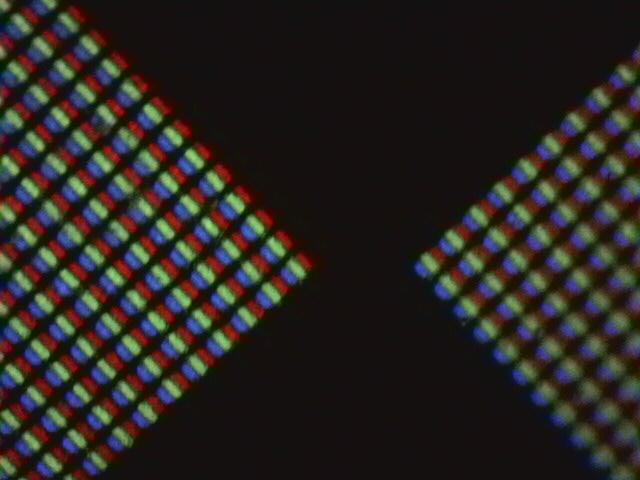
\includegraphics[width=0.9\textwidth]{images/tela_no_microscopio.jpg}
        \caption{Tela do celular ampliada no microscópio.}
    \end{figure}

    \note{
        \begin{columns}[T]
            \begin{column}{0.49\textwidth}
                \scriptsize
                \textbf{Análise da Imagem Ampliada:}
                \begin{itemize}
                    \setlength{\itemsep}{1pt}
                    \item \textbf{A Ilusão Óptica:} O que o usuário enxerga a distância como uma imagem contínua e suave, na verdade é uma matriz discreta de emissores isolados.
                    \item \textbf{Geometria do Pixel:} Cada ponto luminoso (pixel) é composto pela tríade física fixa: uma faixa Vermelha, uma Verde e uma Azul.
                    \item \textbf{Cores Secundárias:} Para gerar Amarelo, o hardware acende os filetes R e G com potência máxima e desliga o B. A mistura ocorre no espaço (retina), não na tela.
                \end{itemize}
            \end{column}

            \begin{column}{0.49\textwidth}    
                \scriptsize
                \textbf{Conexão com Baixo Nível:}
                \begin{itemize}
                    \setlength{\itemsep}{1pt}
                    \item \textbf{Controle de Intensidade:} A variação de cores que vemos na imagem não é o LED mudando de cor, mas sim a variação do brilho relativo (luminância) de cada filete.
                    \item \textbf{Densidade (PPI):} Telas modernas possuem centenas de pixels por polegada, tornando esses filetes imperceptíveis a olho nu, exigindo lentes ou macro.
                    \item \textbf{Analogia Técnica:} O Framebuffer na memória dita diretamente a modulação por largura de pulso (PWM) ou a tensão elétrica que alimenta cada um desses filetes individuais.
                \end{itemize}
            \end{column}
        \end{columns}
    }
\end{frame}

\begin{frame}{Síntese Subtrativa: Modelo CMYK}
    \begin{columns}
        \begin{column}{0.55\textwidth}
            \textbf{Sistemas Subtrativos de Absorção:}

            \begin{itemize}
                \item Aplicado em meios físicos onde a cor \textbf{não tem luz própria} (papel, tintas, corantes).
                \item A tinta funciona como um filtro: ela \textbf{subtrai (absorve)} frequências e reflete o resto.
            \end{itemize}
        \end{column}
        
        \begin{column}{0.45\textwidth}
            \begin{figure}
                \centering
                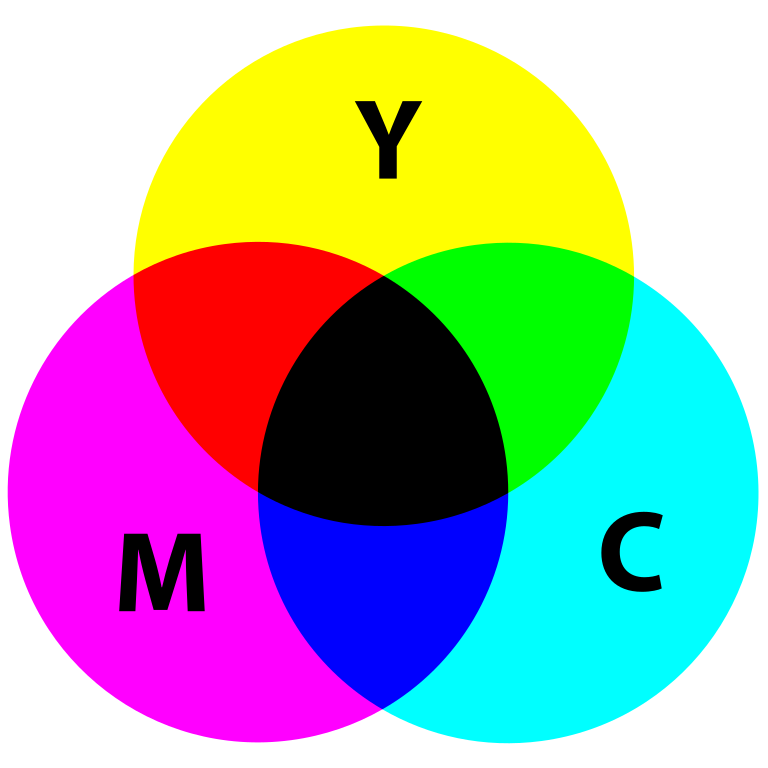
\includegraphics[width=0.9\textwidth]{images/sintese_subtrativa_cmyk.png}
                \caption{Subtração de luz - CMYK.}
            \end{figure}
        \end{column}
    \end{columns}

    \note{
        \begin{columns}[T]
            \begin{column}{0.5\textwidth}
                \scriptsize

                \textbf{Física dos Pigmentos Primários:}
                \begin{itemize}
                    \item \textbf{Ciano} absorve Vermelho (reflete G+B).
                    \item \textbf{Magenta} absorve Verde (reflete R+B).
                    \item \textbf{Amarelo} absorve Azul (reflete R+G).
                \end{itemize}

                \vspace{0.2cm}

                \textbf{A Lógica Prática:}
                \begin{itemize}
                    \setlength{\itemsep}{1pt}
                    \item \textbf{Luz Ambientes:} Para o papel ter cor, ele depende de uma luz externa (branca) batendo nele.
                    \item \textbf{O Filtro:} Quando você joga tinta ciano, você está criando uma barreira química que "engole" os fótons vermelhos da lâmpada do quarto. O que sobra e volta pro seu olho é o Verde e Azul (Ciano).
                \end{itemize}
            \end{column}

            \begin{column}{0.5\textwidth}    
                \scriptsize

                \textbf{Engenharia Gráfica:}
                \begin{itemize}
                    \setlength{\itemsep}{1pt}
                    \item \textbf{O mistério do K:} Explique que "K" vem de \textit{Key Plate} (a placa matriz preta que dava os detalhes e contornos na prensa tradicional).
                    \item \textbf{Problema de Negócio:} Se você imprimir um texto longo usando CMY para fazer preto, o papel sai molhado, enruga, rasga e a impressora gasta 3x mais cartucho. Preto puro resolve isso.
                \end{itemize}

                \textbf{Otimização de Processo (O canal K):}
                \begin{itemize}
                    \item \textbf{Engenharia Química:} Misturar $C+M+Y$ cria um marrom lamacento devido a impurezas.
                    \item \textbf{Custo e Secagem:} Usar a tinta preta ($K$) evita encharcar o papel e reduz drasticamente o custo por página.
                \end{itemize}
            \end{column}
        \end{columns}
    }
\end{frame}

\begin{frame}{O Conflito de Gamut}
    \begin{columns}[T]
        \begin{column}{0.55\textwidth}
            \begin{itemize}
                \item \textbf{O Problema do Mundo Real:}
                \begin{itemize}
                    \item \textbf{Gamut} é o limite físico de cores que um hardware consegue alcançar.
                    \item Tons "neon" ou verdes hiper-saturados do RGB dependem da emissão direta de luz. Pigmentos químicos (CMYK) não conseguem imitar esse brilho.
                \end{itemize}

                \vspace{0.2cm}

                \item \textbf{A Solução via Software:}
                \begin{itemize}
                    \item Quando uma cor da tela está "fora" do limite da impressora, o sistema roda algoritmos de \textbf{Mapeamento de Gamut}.
                \end{itemize}
            \end{itemize}
        \end{column}
        
        \begin{column}{0.45\textwidth}
            \begin{figure}
                \centering
                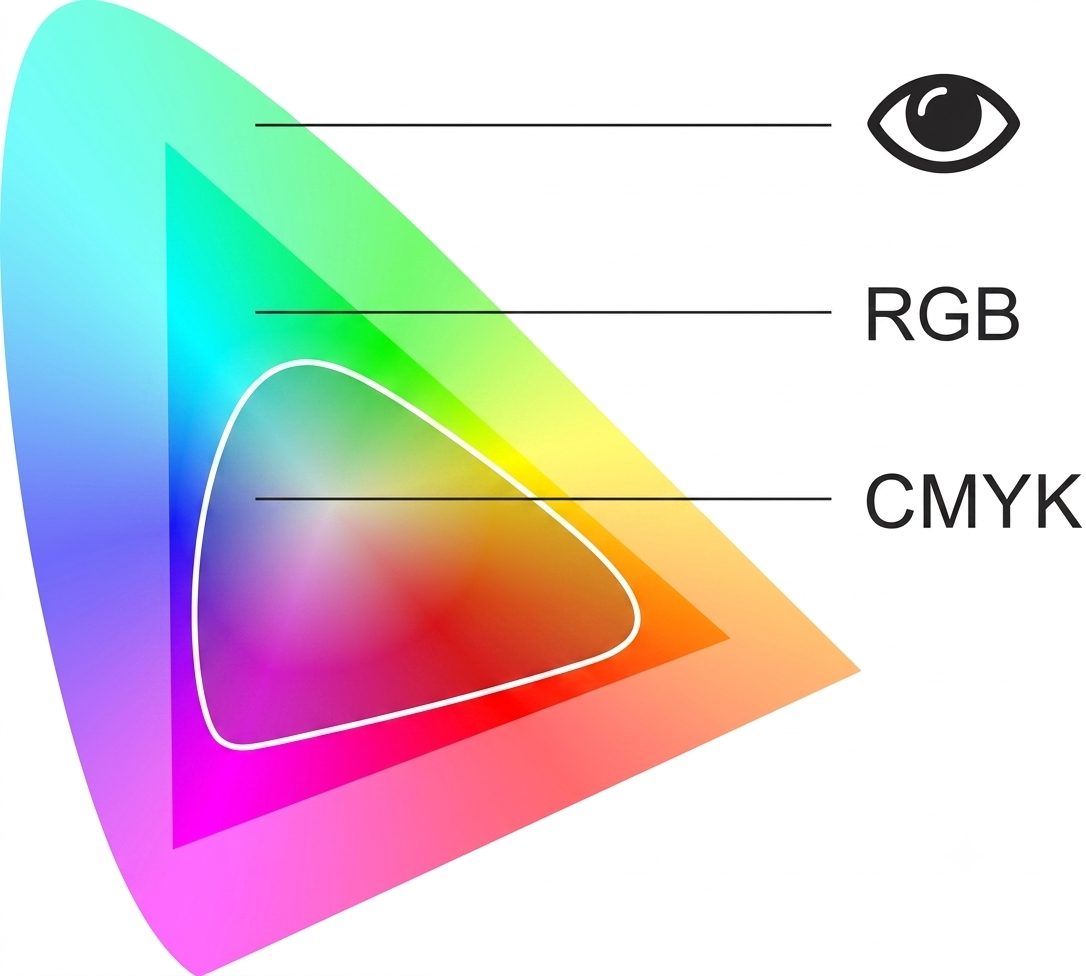
\includegraphics[width=0.9\textwidth]{images/grafico_gamut_cie.png}
                \caption{Interseção e distorção entre os limites RGB e CMYK.}
            \end{figure}
        \end{column}
    \end{columns}

    \note{
        \begin{columns}[T]
            \begin{column}{0.52\textwidth}
                \scriptsize
                \textbf{Leitura do Gráfico (Diagrama CIE):}
                \begin{itemize}
                    \setlength{\itemsep}{0pt}
                    \item \textbf{A Ferradura (Olho):} Representa todo o espectro visível pelo olho humano.
                    \item \textbf{Triângulo (RGB):} O limite que as telas alcançam. \textbf{Polígono interno (CMYK):} O limite da impressão.
                    \item \textbf{Visualização do Conflito:} A área do triângulo RGB que fica de fora do CMYK (como os verdes/azuis no topo) são as cores impossíveis de imprimir, gerando a necessidade do mapeamento.
                \end{itemize}

                \textbf{O Choque de Hardware:}
                \begin{itemize}
                    \setlength{\itemsep}{1pt}
                    \item \textbf{O Susto do Cliente:} Na tela tá um verde neon, na blusa tá um verde fosco.
                    \item \textbf{Limitação da Física:} O pigmento físico simplesmente não reflete aquela frequência de fótons.
                \end{itemize}
            \end{column}

            \begin{column}{0.48\textwidth}    
                \scriptsize
                \textbf{Estratégias de Renderização (CMS):}
                \begin{itemize}
                    \setlength{\itemsep}{1pt}
                    \item \textbf{Perceptual (Fotográfico):} Reduz o gamut inteiro proporcionalmente. Comprime todas as cores da imagem (inclusive as que a impressora conseguiria fazer) para preservar o gradiente e a relação visual entre elas. Evita estouros.
                    \item \textbf{Colorimétrico Relativo:} Faz o \textit{clipping} (poda). Mantém as cores internas idênticas e intocadas. Tudo o que estiver fora do limite é achatado (\textit{clamped}) na borda do gamut. Excelente para logos e cores sólidas exatas, mas destrói degradês finos.
                \end{itemize}
            \end{column}
        \end{columns}   
    }
\end{frame}
% ==========================================
% SEÇÃO 3: MODELOS ORIENTADOS AO USUÁRIO E TRANSMISSÃO
% ==========================================
\section[Modelos]{Modelos de Cor e Transmissão}

\begin{frame}{Modelos Orientados ao Usuário: HSV e HSL}
    \begin{columns}[T]
        \begin{column}{0.55\textwidth}
            \begin{itemize}
                \item \textbf{A Falha Cognitiva do RGB:} O cérebro humano não calcula cores somando intensidades de luz.
                \vspace{0.2cm}
                \item \textbf{Abstração de Uso Prático:}
                \begin{itemize}
                    \item Hue (Matiz).
                    \item Saturation.
                    \item Value / Lightness.
                \end{itemize}
                \vspace{0.2cm}
                \item \textbf{Aplicação em UI/UX:} Base para seletores de cor (\textit{Color Pickers}). O usuário escolhe a tonalidade e depois ajusta a variação de brilho e pureza.
            \end{itemize}
        \end{column}
        
        \begin{column}{0.45\textwidth}
            \begin{figure}
                \centering
                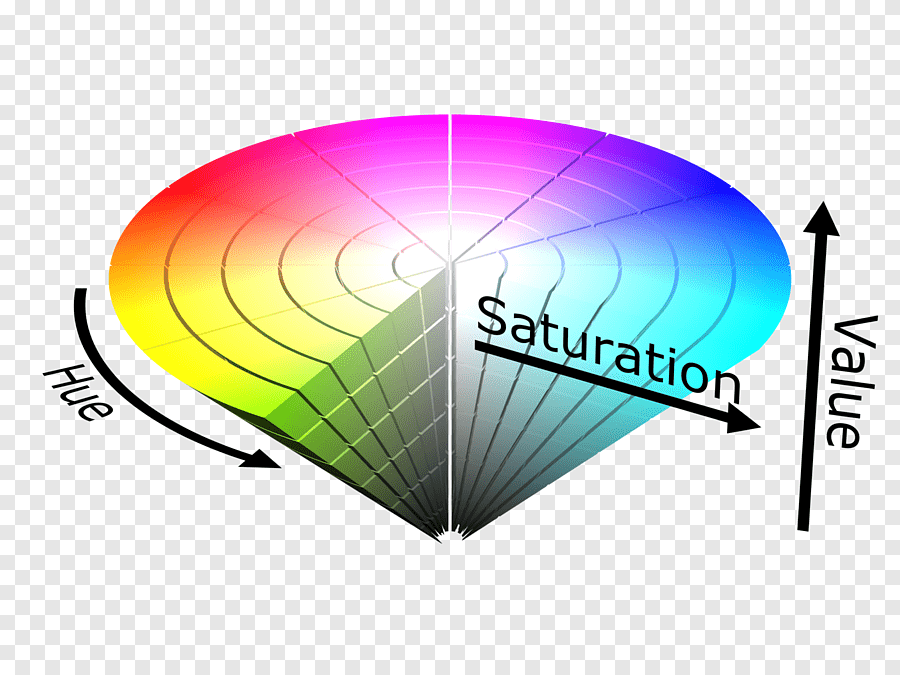
\includegraphics[width=0.9\textwidth]{images/cone_hsv.png}
                \caption{Espaço geométrico tridimensional do modelo HSV.}
            \end{figure}
        \end{column}
    \end{columns}

    \note{
        \begin{columns}[T]
            \begin{column}{0.49\textwidth}
                \scriptsize
                \textbf{RGB vs. HSV:} O RGB é um modelo de hardware, construído para otimizar o envio de sinal elétrico para subpixels na tela. O HSV e o HSL são modelos de software, construídos para alinhar a computação com a cognição visual humana.

                \textbf{Abstração de Uso Prático:}
                \begin{itemize}
                    \setlength{\itemsep}{1pt}
                    \item \textbf{Hue (Matiz):} A cor em si, mapeada em um círculo angular de 0° a 360° (onde 0° é Vermelho, 120° Verde, 240° Azul).
                    \item \textbf{Saturation:} O nível de pureza (0\% cinza absoluto, 100\% cor viva).
                    \item \textbf{Value / Lightness:} A quantidade de luz ou sombra injetada na cor.
                \end{itemize}
            \end{column}

            \begin{column}{0.51\textwidth}    
                \scriptsize
                \textbf{Engenharia de Software (UI):}
                \begin{itemize}
                    \setlength{\itemsep}{1pt}
                    \item \textbf{Aplicação em UI/UX:} Base para seletores de cor (\textit{Color Pickers}). O usuário escolhe a tonalidade e depois ajusta a variação de brilho e pureza.
                    \item \textbf{Conversão em Back-end:} Quando o usuário define a cor HSV interface, o programa converte para RGB antes de despachar para o barramento.
                \end{itemize}
                O cérebro humano não calcula cores somando intensidades de luz (ex: descobrir a mistura exata de R, G e B para gerar um tom de marrom).

                No HSV, $V=100\%$ é a cor pura (usado no Photoshop e Figma); no HSL, a cor pura fica em $L=50\%$, pois $L=100\%$ vira branco absoluto (padrão nativo na Web/CSS). O HSL é ideal na programação para criar paletas e \textit{Dark Mode} alterando apenas a variável $L$ aritmeticamente, sem quebrar o vetor de cor.
            \end{column}
        \end{columns}   
    }
\end{frame}

\begin{frame}{Transmissão e Processamento Cognitivo: YIQ e Cores Oponentes}
    \begin{columns}[T]
        \begin{column}{0.55\textwidth}
            \begin{itemize}
                \item \textbf{O Modelo YIQ e Engenharia de Software:}
                \begin{itemize}
                    \item \textbf{Criado para retrocompatibilidade.}
                    \item \textbf{Compressão de Banda:} O olho humano foca em detalhes no brilho ($Y$), não na cor.
                \end{itemize}

                \item \textbf{A Engenharia Biológica (Cores Oponentes):}
                \begin{itemize}
                    \item A retina converte os sinais de R, G e B em três eixos diferenciais de voltagem.
                \end{itemize}
            \end{itemize}
        \end{column}
        
        \begin{column}{0.45\textwidth}
            \begin{figure}
                \centering
                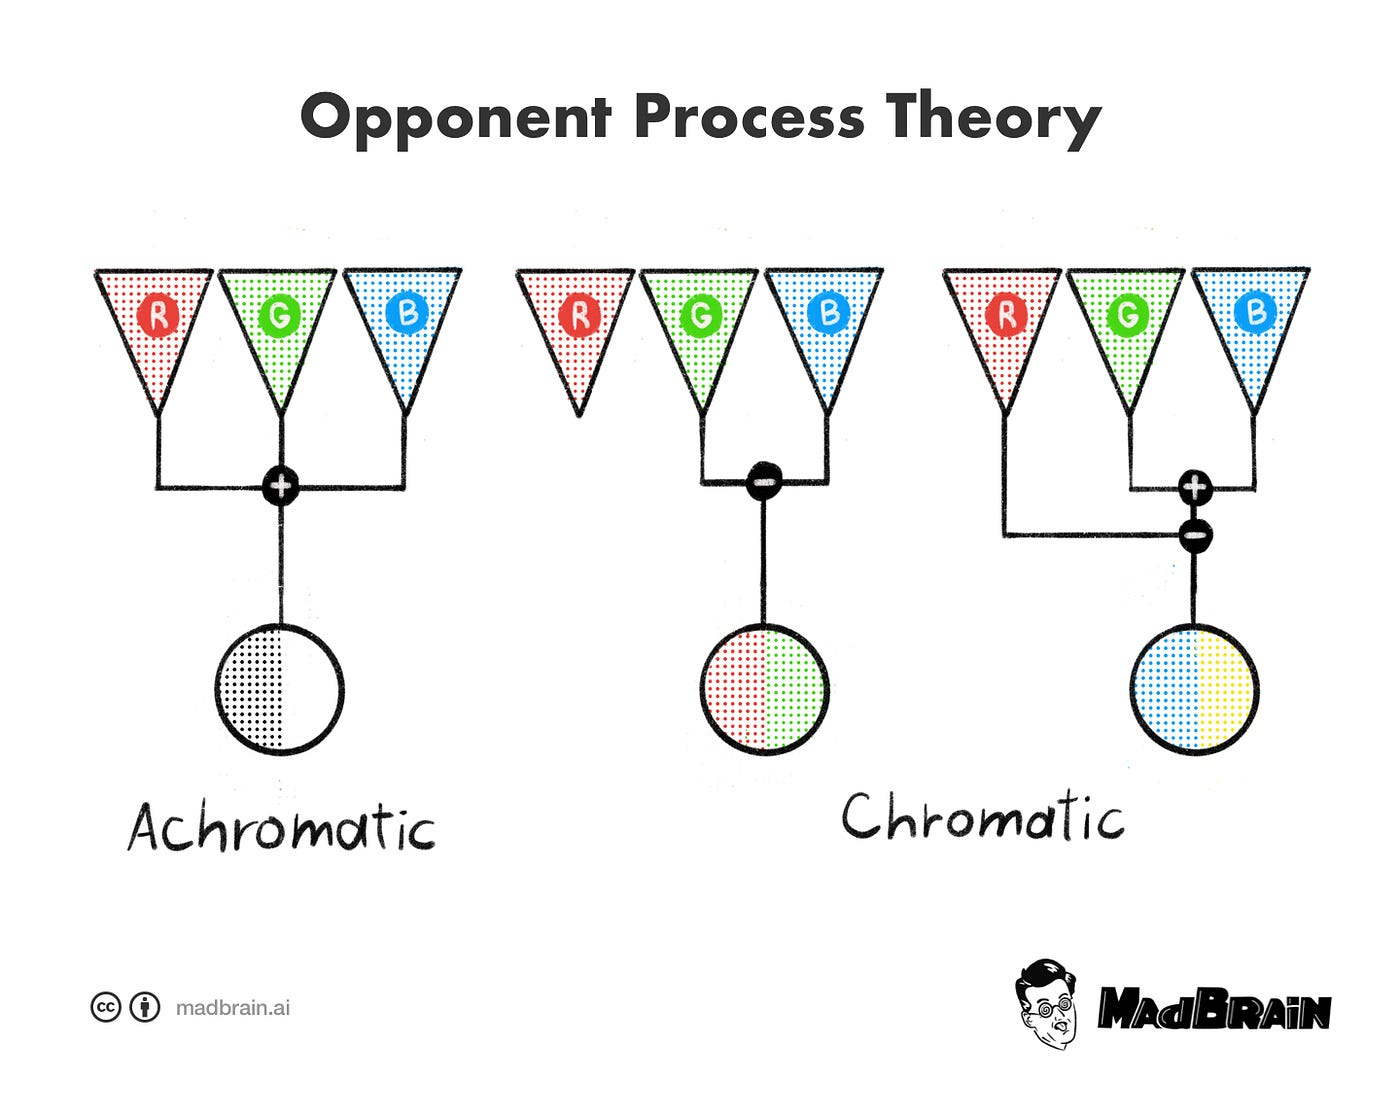
\includegraphics[width=0.9\textwidth]{images/teoria_oponentes.jpg}
                \caption{Esquema dos canais neurais oponentes e compressão de sinal.}
            \end{figure}
        \end{column}
    \end{columns}

    \note{
        \begin{columns}[T]
            \begin{column}{0.49\textwidth}
                \scriptsize
                \textbf{Otimização de Hardware e Banda:}
                \begin{itemize}
                    \setlength{\itemsep}{1pt}
                    \item \textbf{Subamostragem de Crominância:} O modelo YIQ é o ancestral direto dos formatos modernos de compressão de vídeo como YCbCr (usado em JPEG e MP4). O software descarta dados de cor porque a nossa acuidade visual para detalhes finos está concentrada quase que inteiramente na escala de cinza ($Y$).
                    \item O YIQ foi criado para retrocompatibilidade: TVs P\&B liam apenas o canal Y (Luminância/Brilho). TVs coloridas decodificavam I e Q (Crominância/Cor).
                    O olho humano foca em detalhes no brilho ($Y$), não na cor. Isso permitiu que engenheiros de transmissão reduzissem a largura de banda de $I$ e $Q$ pela metade sem perda de qualidade percebida.
                \end{itemize}
            \end{column}

            \begin{column}{0.51\textwidth}    
                \scriptsize
                \textbf{Mecânica Neurofisiológica:}
                \begin{itemize}
                    \setlength{\itemsep}{1pt}
                    \item \textbf{Fadiga de Receptores (Afterimage):} Olhar fixamente para uma imagem verde forte satura as células do oponente Verde. Ao olhar para uma parede branca, após isso, o receptor fadigado falha em disparar o sinal verde, fazendo com que o eixo oposto (Vermelho) dispare livremente. Gerando a ilusão de ver a mesma imagem em vermelho.
                \end{itemize}

                \textbf{A Engenharia Biológica (Cores Oponentes):}
                \begin{itemize}
                    \item A retina converte os sinais de R, G e B em três eixos diferenciais de voltagem: Vermelho-Verde, Azul-Amarelo e Claro-Escuro.
                    \item Como um sinal elétrico inibe o outro no mesmo canal, o cérebro não consegue processar "verde-avermelhado".
                \end{itemize}
            \end{column}
        \end{columns}   
    }
\end{frame}
% % ==========================================
% SEÇÃO 4: MATEMÁTICA E PROCESSAMENTO
% ==========================================
\section[Processamento]{Matemática e Processamento}

\begin{frame}{Transformações de Espaço e o Histograma}
    \begin{itemize}
        \item \textbf{Matrizes de Transformação:}
        \begin{itemize}
            \item A conversão entre espaços de cor não é arbitrária; ela ocorre via multiplicação de matrizes por vetores de pixels $[R, G, B]^T$.
            \item \textbf{CIE XYZ:} Espaço matemático universal usado como "ponte" de tradução entre hardwares diferentes.
        \end{itemize}
        
        \vspace{0.2cm}
        
        \item \textbf{O Histograma como Array de Dados:}
        \begin{itemize}
            \item É um vetor de contagem estatística discreta. Para imagens de 8 bits, cria-se um array de 256 posições (\textit{bins}).
            \item Varre-se a matriz de pixels incrementando o índice correspondente à intensidade encontrada.
        \end{itemize}
        
        \vspace{0.2cm}
        
        \item \textbf{Engenharia de Algoritmos (CBIR):}
        \begin{itemize}
            \item Sistemas de busca reversa de imagens comparam a distância euclidiana ou a interseção entre vetores de histogramas para medir similaridade cromática.
        \end{itemize}
    \end{itemize}

    \note{
        \begin{columns}[T]
            \begin{column}{0.49\textwidth}
                \scriptsize
                \textbf{Pipeline de Álgebra Linear:}
                \begin{itemize}
                    \setlength{\itemsep}{1pt}
                    \item \textbf{Pipeline de GPU:} A conversão RGB para XYZ utiliza uma matriz $3 \times 3$ fixa com coeficientes baseados no observador padrão. Como essa operação é uma transformação linear pura e independente para cada pixel, ela é paralelizada nativamente em Shaders dentro da GPU, permitindo processamento em tempo real de fluxos de vídeo em alta resolução.
                \end{itemize}
            \end{column}

            \begin{column}{0.49\textwidth}    
                \scriptsize
                \textbf{Manipulação Estatística:}
                \begin{itemize}
                    \setlength{\itemsep}{1pt}
                    \item \textbf{Equalização de Histograma:} Algoritmos de melhoria de contraste usam a Função de Distribuição Acumulada (CDF) do histograma para redistribuir as frequências de pixels. Áreas muito concentradas (subexpostas ou superexpostas) têm seus valores espalhados linearmente por todo o array de 0 a 255, maximizando a entropia e o contraste da imagem de forma automatizada.
                \end{itemize}
            \end{column}
        \end{columns}   
    }
\end{frame}
% ==========================================
% SEÇÃO 5: IMPLEMENTAÇÃO E COMPUTAÇÃO GRÁFICA AVANÇADA
% ==========================================
\section[Implementação]{Implementação e Computação Gráfica Avançada}

\begin{frame}{Cores em OpenGL e o Canal Alpha}
    \begin{columns}[T]
        \begin{column}{0.55\textwidth}
            \textbf{Alocação de Memória (VRAM):}
            \begin{itemize}
                \item Em arquiteturas de 32 bits, cada pixel é um array contíguo de 4 bytes na GPU: \texttt{[R, G, B, A]}.
                \item O canal \textbf{Alpha} mapeia a opacidade escalar como um ponto flutuante de \texttt{0.0} (transparente) a \texttt{1.0} (opaco).
            \end{itemize}
            
                \vspace{0.2cm}
            
                \textbf{O Algoritmo de Blending:}
            \begin{itemize}
                \item Para renderizar transparência, o hardware mistura a cor do novo fragmento (\textit{Source}) com a cor já gravada no Framebuffer (\textit{Destination}).
            \end{itemize}
        \end{column}
        
        \begin{column}{0.45\textwidth}
            \begin{figure}
                \centering
                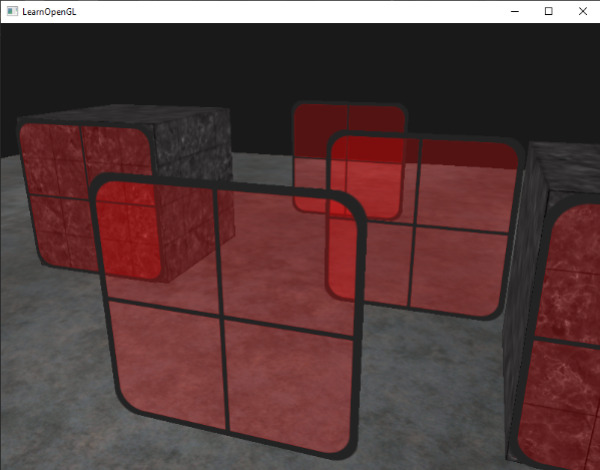
\includegraphics[width=0.9\textwidth]{images/mecanismo_blending.jpg}
                \caption{Operação de Alpha Blending diretamente nos registradores do Framebuffer.}
            \end{figure}
        \end{column}
    \end{columns}

    \note{
        \begin{columns}[T]
            \begin{column}{0.49\textwidth}
                \scriptsize
                \textbf{Gargalo do Z-Buffer:}
                \begin{itemize}
                    \setlength{\itemsep}{1pt}
                    \item \textbf{A Ordem de Renderização:} Objetos opacos podem ser desenhados em qualquer ordem porque o teste de profundidade (Z-buffer) descarta pixels tapados. Objetos transparentes que usam blending quebram essa lógica. A equação matemática não é comutativa; se o programador desenhar o fundo após o objeto transparente, o cálculo falha.
                \end{itemize}
            \end{column}

            \begin{column}{0.49\textwidth}    
                \scriptsize
                \textbf{Solução em Software:}
                \begin{itemize}
                    \setlength{\itemsep}{1pt}
                    \item \textbf{Ordenação de Polígonos:} Engines de jogos precisam ordenar todas as geometrias translúcidas da cena com base na distância da câmera (do mais distante para o mais próximo) a cada frame antes de enviar os dados de vértice para os Draw Calls da API gráfica.
                \end{itemize}
            \end{column}
        \end{columns}   
    }
\end{frame}

\begin{frame}{Técnicas Avançadas de Realismo Cromático}
    \begin{columns}[T]
        \begin{column}{0.5\textwidth}
            \textbf{Lightmaps (Iluminação Pré-Calculada):}
            \begin{itemize}
                \item Calcular equações de raio (\textit{Ray Tracing}) em tempo real a 60 FPS é computacionalmente proibitivo para hardware comum.
            \end{itemize}
            
            \vspace{0.2cm}
            
            \textbf{Sub-Surface Scattering (SSS):}
            \begin{itemize}
                \item Algoritmo que simula a física de materiais translúcidos (pele, cera, folhas).
            \end{itemize}
        \end{column}
        
        \begin{column}{0.5\textwidth}
            \begin{figure}
                \centering
                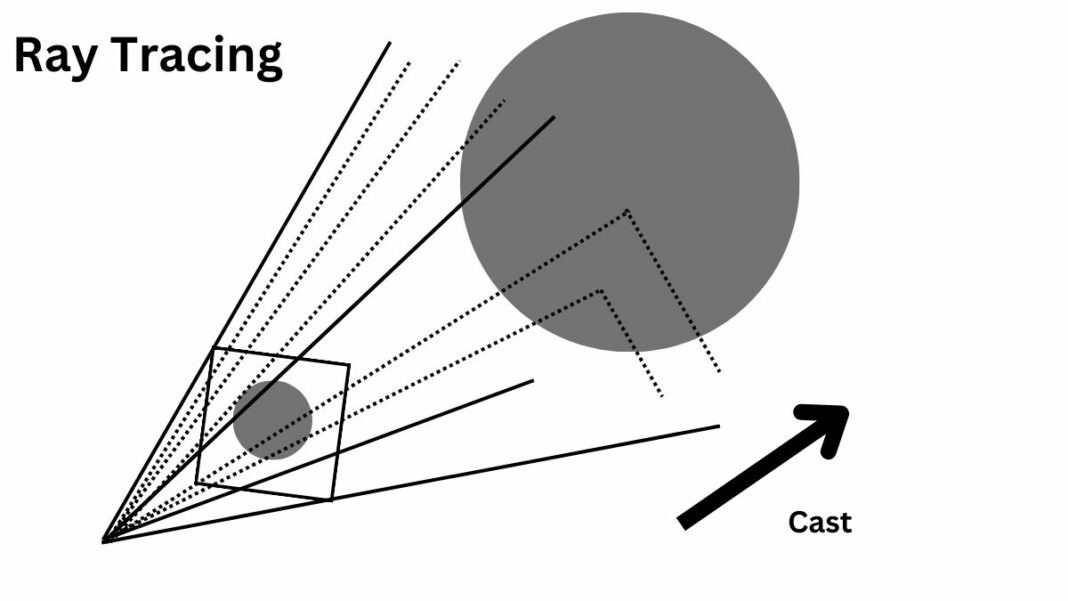
\includegraphics[width=0.9\textwidth]{images/subsurface_scattering_demo.jpg}
                \caption{Comportamento físico dos vetores de luz na técnica de SSS.}
            \end{figure}
        \end{column}
    \end{columns}

    \note{
        \begin{columns}[T]
            \begin{column}{0.49\textwidth}
                \scriptsize
                \textbf{Otimização de Textura:}
                \begin{itemize}
                    \setlength{\itemsep}{1pt}
                    \item \textbf{Custo de Memória:} O uso de Lightmaps zera o custo de processamento de shaders de iluminação dinâmica na CPU/GPU durante a execução do software. O trade-off é estritamente o consumo de VRAM, já que o jogo precisa carregar texturas adicionais de alta resolução contendo apenas o mapa de sombras mapeado na malha.
                \end{itemize}

                \textbf{Sub-Surface Scattering (SSS):}
                \begin{itemize}
                    \item Simula a física de materiais translúcidos (pele, cera, folhas).
                    \item Os fótons não ricocheteiam na superfície; eles penetram o material, sofrem desvios internos e saem em outra coordenada.
                \end{itemize}
            \end{column}

            \begin{column}{0.49\textwidth}    
                \scriptsize
                \textbf{Física de Shaders (SSS):}
                \begin{itemize}
                    \setlength{\itemsep}{1pt}
                    \item \textbf{O Efeito Plástico:} Sem o algoritmo de SSS, a iluminação aproximada clássica (Lambert/Phong) trata a geometria como opaca pura. Em bordas finas retroiluminadas (como uma orelha contra o sol), a ausência do espalhamento interno faz a pele parecer plástico escuro e sem vida, destruindo o fotorrealismo.
                \end{itemize}

                \textbf{Lightmaps (Iluminação Pré-Calculada):}
                \begin{itemize}
                    \item \textbf{Solução:} As sombras e rebatimentos de luz estáticos são processados na compilação (\textit{Baking}) e salvos como texturas normais injetadas no segundo canal de UV da malha.
                \end{itemize}
            \end{column}
        \end{columns}   
    }

\end{frame}





\begin{frame}{O Algoritmo de Dithering e a Ilusão Cromática}
    \begin{columns}[T]
        \begin{column}{0.55\textwidth}
            \textbf{Quantização e Redução de Cores:}
            \begin{itemize}
                \item Técnica matemática para simular maior profundidade de cor (bits por pixel) em hardwares com paletas severamente limitadas.
                \item Utiliza padrões geométricos de pixels ou difusão de erro para enganar a percepção humana.
            \end{itemize}
            
            \vspace{0.2cm}
            
            \textbf{O Papel do Hardware Analógico (CRT):}
            \begin{itemize}
                \item A imperfeição física dos monitores CRT atuava como um filtro passa-baixa natural, fundindo os pixels em degradês suaves.
            \end{itemize}
        \end{column}
        
        \begin{column}{0.45\textwidth}
            \begin{figure}
                \centering
                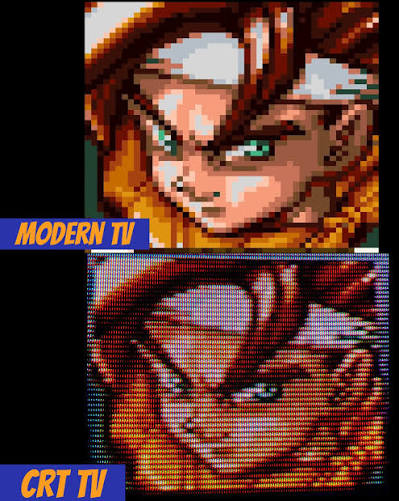
\includegraphics[width=0.7\textwidth]{images/chrono_trigger.png}
                \caption{Fusão óptica de pseudo-cores através de entrelaçamento de pixels em malhas CRT.}
            \end{figure}
        \end{column}
    \end{columns}

    \note{
        \begin{columns}[T]
            \begin{column}{0.49\textwidth}
                \scriptsize
                \textbf{Difusão de Erro (Floyd-Steinberg):}
                \begin{itemize}
                    \setlength{\itemsep}{1pt}
                    \item \textbf{A Matemática:} O algoritmo calcula a diferença entre a cor original do pixel e a cor mais próxima disponível na paleta. Esse erro residual é distribuído/difundido para os pixels vizinhos ainda não processados usando uma matriz de pesos.
                \end{itemize}
            \end{column}

            \begin{column}{0.49\textwidth}    
                \scriptsize
                \textbf{Anacronismo Digital (LCD/OLED):}
                \begin{itemize}
                    \setlength{\itemsep}{1pt}
                    \item \textbf{Quebra da Ilusão:} Telas modernas exibem pixels estritos com matrizes nítidas e sem vazamento de luz. Sem o desfoque do CRT, os padrões de dithering tornam-se artefatos de ruído visíveis. Engines modernas aplicam filtros de interpolação para restaurar o efeito pretendido originalmente.
                \end{itemize}
            \end{column}
        \end{columns}   
    }
\end{frame}



% ==========================================
% SEÇÃO 4: TECNOLOGIAS DE TELAS E DISPLAYS
% ==========================================
\section{Tecnologias de Displays}

% --- SLIDE 1: IPS ---
\begin{frame}{Telas IPS: Alinhamento de Cristais e Precisão Cromática}
    \begin{columns}[T]
        \begin{column}{0.55\textwidth}
            \small
            \begin{itemize}
                \item \textbf{Orientação em Plano (In-Plane):} Os cristais líquidos giram paralelamente ao plano do painel quando submetidos a um campo elétrico.
                \vspace{0.2cm}
                \item \textbf{Ângulo de Visão Estendido:} Consistência de cor e contraste mesmo em observações oblíquas periféricas (até 178°).
                \vspace{0.2cm}
                \item \textbf{Fidelidade Cromática:} Modelo padrão para calibração profissional em design gráfico, engenharia de interface e fotografia.
            \end{itemize}
        \end{column}
        
        \begin{column}{0.45\textwidth}
            \begin{figure}
                \centering
                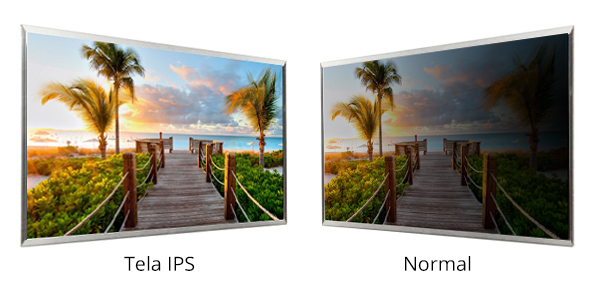
\includegraphics[width=0.9\textwidth]{images/ips.png}
                \caption{Mecanismo de rotação paralela dos cristais IPS.}
            \end{figure}
        \end{column}
    \end{columns}

    \note{
        \footnotesize
        \begin{columns}[T]
            \begin{column}{0.49\textwidth}
                \textbf{Física Óptica do Painel:}
                \begin{itemize}
                    \setlength{\itemsep}{1pt}
                    \item \textbf{Bloqueio de Luz:} Como os cristais apenas barram a luz polarizada de um backlight sempre ativo, o fechamento físico dos canais não é perfeito.
                    \item \textbf{Contraste Nativo Baixo:} Painéis IPS convencionais raramente ultrapassam a razão estática de 1000:1, fazendo com que tons pretos pareçam cinza escuro em ambientes de baixa iluminação.
                \end{itemize}
            \end{column}

            \begin{column}{0.49\textwidth}    
                \textbf{Limitações de Hardware:}
                \begin{itemize}
                    \setlength{\itemsep}{1pt}
                    \item \textbf{Backlight Bleeding:} Defeito estrutural ou pressão mecânica excessiva na carcaça que permite o escape de luz pelas bordas físicas da tela.
                    \item \textbf{IPS Glow:} Fenômeno óptico difuso onde o brilho do fundo parece flutuar dependendo do ângulo de visão, muito visível nos cantos de displays grandes a distâncias curtas.
                \end{itemize}
            \end{column}
        \end{columns}
    }
\end{frame}

% --- SLIDE 2: MINI-LED ---
\begin{frame}{Telas Mini-LED: Evolução do Backlight e Alto Brilho}
    \begin{columns}[T]
        \begin{column}{0.55\textwidth}
            \small
            \begin{itemize}
                \item \textbf{Retroiluminação Avançada:} Substitui as lâmpadas de borda tradicionais por milhares de diodos minúsculos dispostos atrás da matriz LCD.
                \vspace{0.2cm}
                \item \textbf{Atenuação Local (FALD):} Agrupamento dos LEDs em centenas ou milhares de zonas controladas independentemente por software.
                \vspace{0.2cm}
                \item \textbf{Pico de Luminância:} Excelente capacidade para HDR agressivo, alcançando níveis de brilho muito superiores ao OLED comercial.
            \end{itemize}
        \end{column}
        
        \begin{column}{0.45\textwidth}
            \begin{figure}
                \centering
                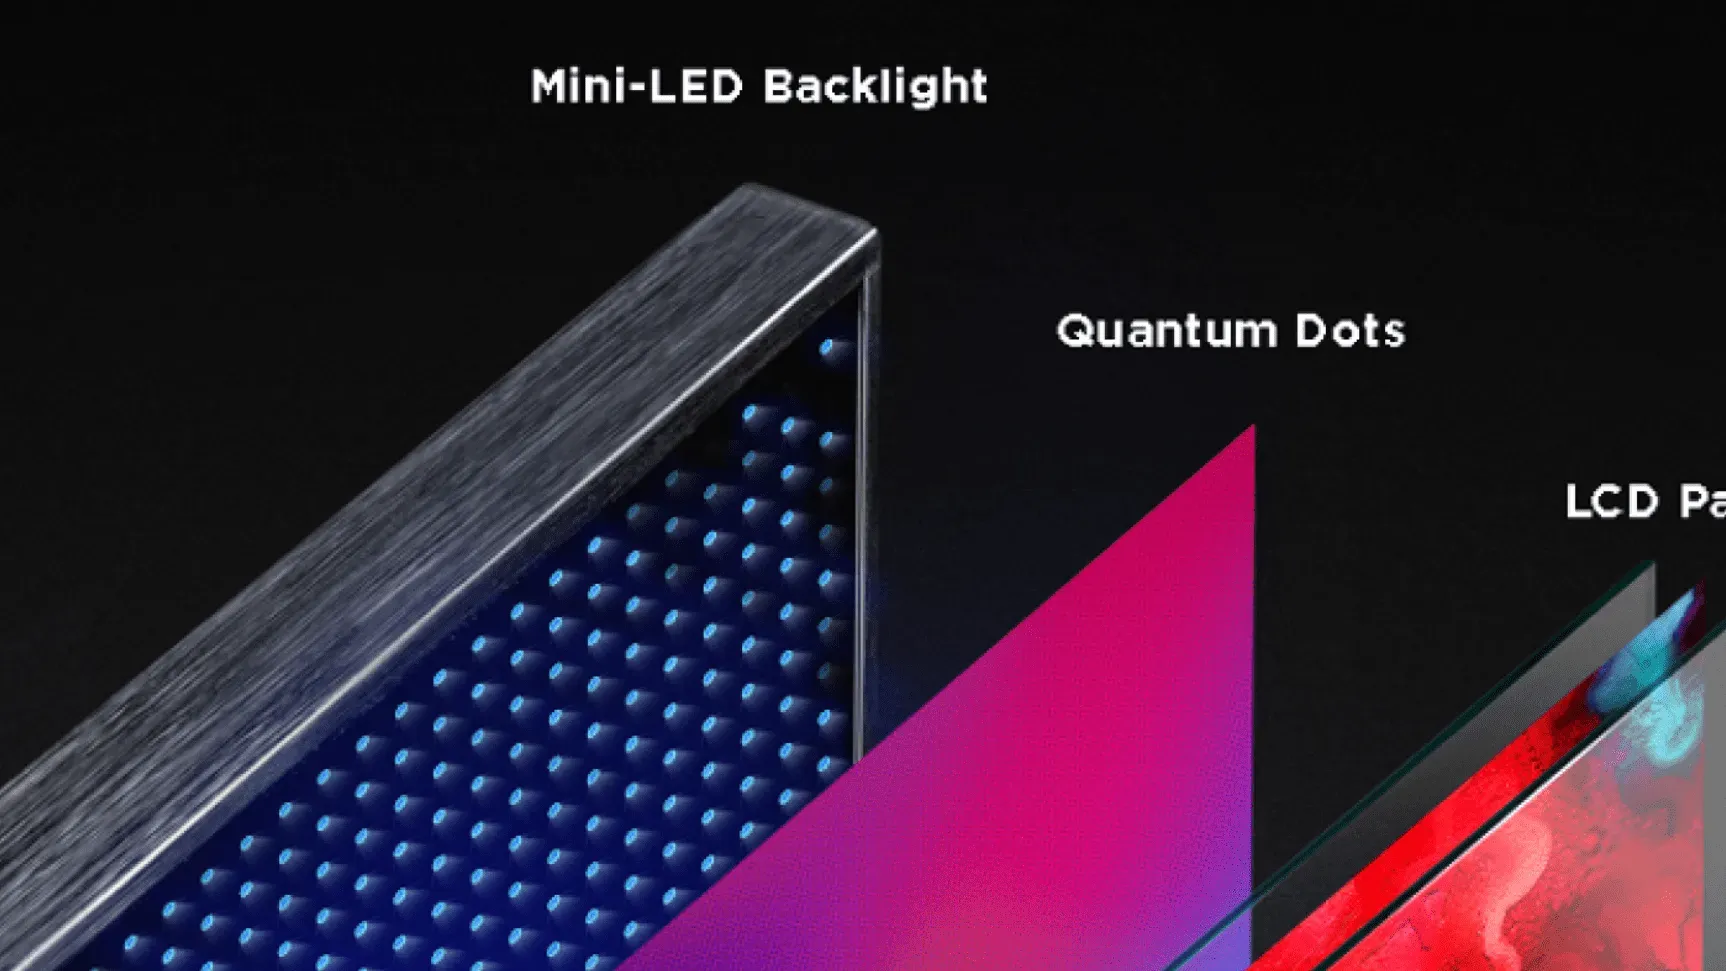
\includegraphics[width=0.9\textwidth]{images/min_led.png}
                \caption{Zonas de retroiluminação em matriz Mini-LED.}
            \end{figure}
        \end{column}
    \end{columns}

    \note{
        \footnotesize
        \begin{columns}[T]
            \begin{column}{0.49\textwidth}
                \textbf{Engenharia de Iluminação:}
                \begin{itemize}
                    \setlength{\itemsep}{1pt}
                    \item \textbf{Mecanismo:} Une a durabilidade e estabilidade química dos compostos inorgânicos (sem risco de burn-in) à modulação espacial de contraste.
                    \item \textbf{O Efeito Blooming:} Limitação física decorrente do desalinhamento de resolução entre a matriz de LEDs (zonas) e a matriz de subpixels LCD. Objetos brilhantes pequenos em fundos pretos geram um "halo" ou vazamento de luz indesejado.
                \end{itemize}
            \end{column}

            \begin{column}{0.49\textwidth}    
                \textbf{Algoritmos de Controle:}
                \begin{itemize}
                    \setlength{\itemsep}{1pt}
                    \item \textbf{Latência de Shaders:} O driver de hardware precisa analisar o frame de entrada e calcular o mapa de atenuação para as zonas de iluminação em tempo real. Algoritmos mal otimizados geram atraso perceptível na mudança de brilho (\textit{luminance lag}).
                \end{itemize}
            \end{column}
        \end{columns}
    }
\end{frame}

% --- SLIDE 3: OLED ---
\begin{frame}{Telas OLED: Emissão Direta e Contraste Absoluto}
    \begin{columns}[T]
        \begin{column}{0.55\textwidth}
            \small
            \begin{itemize}
                \item \textbf{Matriz Autoemissiva:} Cada pixel é composto por diodos orgânicos que emitem sua própria luz sob corrente elétrica.
                \vspace{0.2cm}
                \item \textbf{Contraste Infinito:} A representação do preto digital ($0,0,0$) desliga o emissor por completo.
                \vspace{0.2cm}
                \item \textbf{Tempo de Resposta:} Transição de estado quase instantânea (sub-milissegundo), eliminando rastros visíveis (\textit{ghosting}).
            \end{itemize}
        \end{column}
        
        \begin{column}{0.45\textwidth}
            \begin{figure}
                \centering
                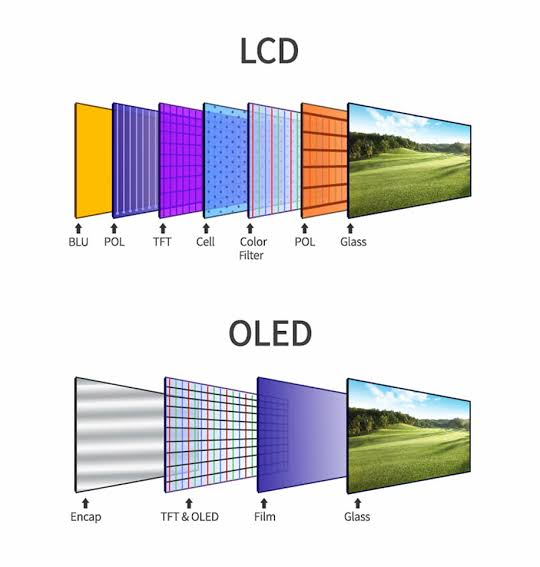
\includegraphics[width=0.9\textwidth]{images/oled.png}
                \caption{Funcionamento de subpixels autoemissivos OLED.}
            \end{figure}
        \end{column}
    \end{columns}

    \note{
        \footnotesize
        \begin{columns}[T]
            \begin{column}{0.49\textwidth}
                \textbf{Física do Estado Sólido:}
                \begin{itemize}
                    \setlength{\itemsep}{1pt}
                    \item \textbf{Arquitetura:} Elimina a necessidade de uma camada difusora e de um backlight centralizado, reduzindo drasticamente a espessura do painel.
                    \item \textbf{O Problema do Burn-in:} Degradação fotoquímica diferencial dos materiais orgânicos. O subpixel azul possui menor eficiência e exige maior corrente, acelerando seu desgaste sob imagens estáticas.
                \end{itemize}
            \end{column}

            \begin{column}{0.49\textwidth}    
                \textbf{Controle de Baixo Nível:}
                \begin{itemize}
                    \setlength{\itemsep}{1pt}
                    \item \textbf{Modulação de Brilho:} Telas OLED frequentemente utilizam PWM (Modulação por Largura de Pulso) para controlar o brilho, o que pode causar cintilação perceptível (\textit{flicker}) e fadiga ocular em frequências baixas.
                    \item \textbf{Eficiência Energética:} O consumo é dinâmico e diretamente proporcional à luminância média da imagem (APL - \textit{Average Picture Level}), tornando o \textit{Dark Mode} uma otimização de hardware real.
                \end{itemize}
            \end{column}
        \end{columns}
    }
\end{frame}

\end{document}
